\chapter{Fundamentals}

\section{Human Action Recognition}
In \textit{Human Action Recognition}, often referred to simply by its acronym \textit{HAR}, the task is to attach a label of an \textit{action} to a signal, be it an image, a video or a set of other sensor values.
Thus, HAR is a \textit{classification} problem where the classes are human actions.
It is important to understand that HAR recognizes the action after it is completed, as opposed to \textit{action prediction} which tries to predict the action while it is still happening \cite{kong_human_2018}.

Typical use-cases of Human Action Recognition consists of evaluating human behaviour, for example in a warehouse context \cite{reining_towards_2018}, or analyzing video surveillance footage \cite{htike_human_2014}.
An example of simple actions performed by multiple subjects is provided in \fref{fig:simple-actions}.

\begin{figure}[htb!]
    \centering
    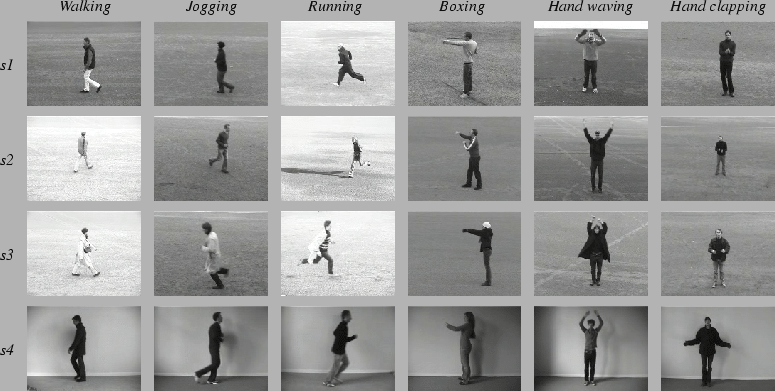
\includegraphics[width=0.8\textwidth]{simple-actions.png}
    \caption{Example of six actions performed by four different subjects, annotated with their corresponding label (top). Image taken from \cite{laptev_learning_2008} }
    \label{fig:simple-actions}
\end{figure}

\subsection{Action Granularity}
When discussing \textit{action}, it should be noted that there are different interpretations, not only of what consists an action but also how finely they should be specified.
As an illustration, consider an image of a person waving with her left hand at the camera.
It is not inherently clear whether the label attached to this action should be \textit{waving}, \textit{raising left arm} or else.
This is why the choice of labels is often domain specific.

According to \cite{zhang_review_2017}, human actions can be categorized into three levels, referred to as \textit{action primitives, activities and interactions}.
\textit{Action primitives} consists of actions where one part of the body is performing the actions.
For example, \textit{waving} or \textit{clapping} would constitute action primitives since a specific part of the body is responsible.
In contrast, \textit{activities} are actions where the whole body is involved in performing the action.
As an example, consider \textit{jumping} or \textit{jogging}.
When considering actions performed involving objects or other persons, i.e. \textit{shaking hands} or \textit{throwing a ball}, \cite{zhang_review_2017} categorize these actions as \textit{interactions}.

\subsection{Video-based HAR}
When considering HAR on video clips, some domain-specific problems arise, which are outlined in \cite{zhang_review_2017}.

Firstly, depending on the camera and recording technique used, the background of the image can be highly dynamic.
This means that the amount of information irrelevant for identifying the action can be very high and might change constantly.
As an example, consider a video filmed with a hand-held modern smart phone.
Because the camera is not stationary, the background will shift while recording.
Also, depending on the scene, illumination changes and occlusion of the human subject might occur.

Secondly, different actions can have similar visual shapes.
Consider \textit{talking on the phone} and \textit{military salute}.
In both cases, the dominant hand is positioned at the side of the subjects head.
Depending on factors like image quality, the subjects rotation towards the camera etc. these two actions might be hard to differentiate.
Also, consider \textit{walking} and \textit{running}.
It is not inherently clear where the boundary between these two classes are, i.e. up to which point is a subject still \textit{walking} and when does the subject begin to \textit{run}?
This problem is referred to as \textit{interclass similarity}.
Another similar problem is \textit{intraclass variation}, where the same action performed by different subjects might vary in its visual representation.
As an example, consider \textit{throwing a ball}.
The scene will differ a lot when considering different clothing of the subject, different shape and color of the ball as well as different contexts where the action is happening, i.e. in a backyard, in a baseball stadium etc.
Also, performing actions at different intensities can alter their appearence, for example \textit{running} can be performed at slow to high speed and might even involve small jumps \cite{kong_human_2018}.

Thirdly, \cite{zhang_review_2017} mention \textit{group activities}.
When there are multiple subjects performing actions in a frame, it can be difficult to differentiate between many individual actions and a group action.
An example would be the difference between \textit{running} and \textit{playing football}.
Not only is a lot of context necessary to be able to determine a group activity but also to determine which subjects are part of the group activity and which are not.
Consider the case where, in a single frame, two subjects are playing football and two subjects are sitting, reading a book.
No single label is able to fully describe the human actions present in the image.
Thus, a sizeable portion of literature focuses on single human, single action problems.

\section{Pose Estimation}

\begin{figure}[htb!]
    \centering
    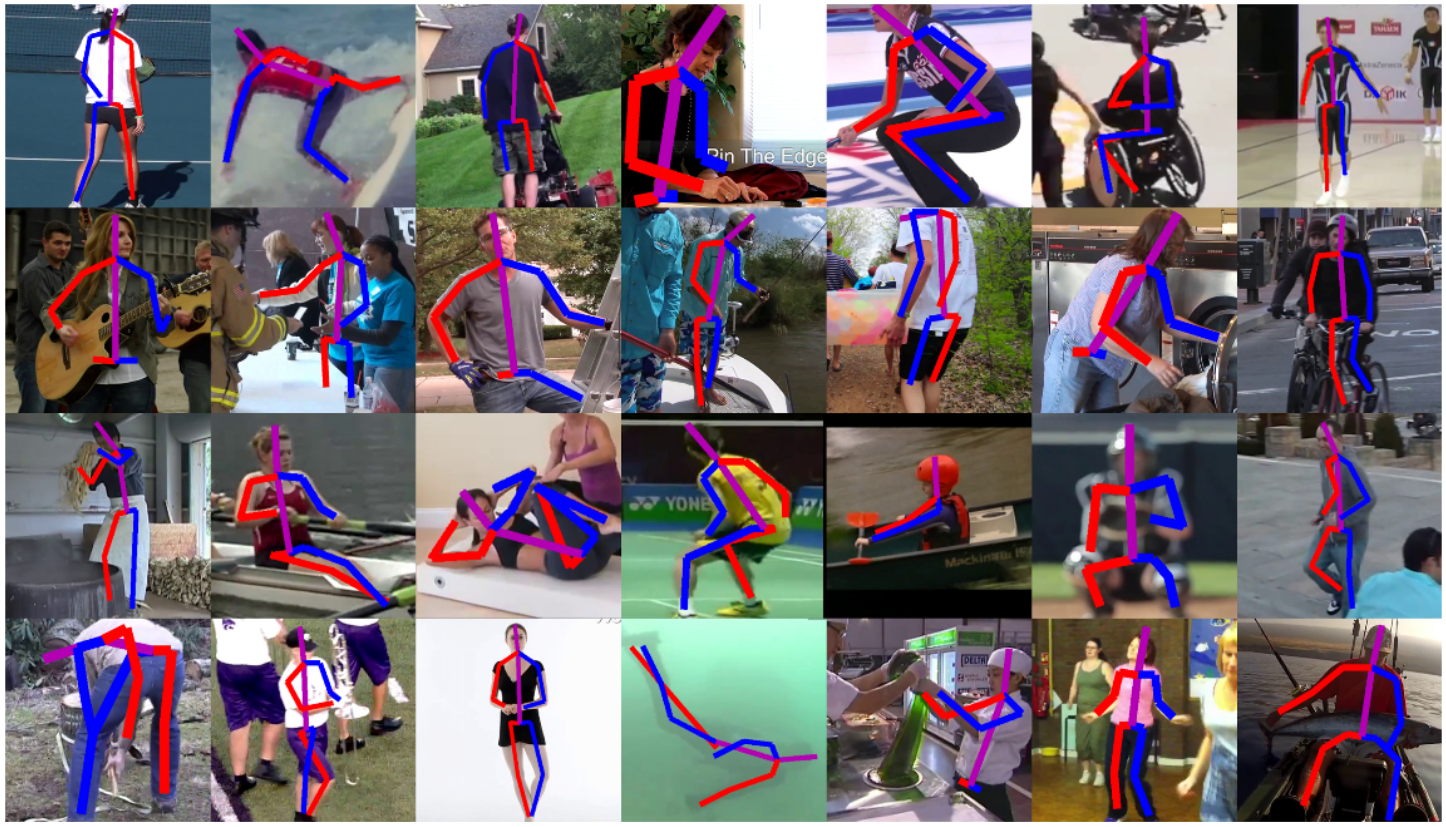
\includegraphics[width=0.9\textwidth]{tree-pose.png}
    \caption{Examples of human pose estimation. The pose is represented using a tree structure of joint positions, forming a skeleton. Image taken from \cite{newell_stacked_2016}}
    \label{fig:tree-skeleton}
\end{figure}

Pose estimation is defined by extracting the coordinates of human joints from an image or from other signals.
In this thesis, however, the main focus is performing pose estimation using image-based methods.
The joint positions are then often represented in a tree structure representing a skeleton.
See \fref{fig:tree-skeleton} for an example.

Such a representation of the human pose is useful in a lot of scenarios.
Action recognition, presented previously, often incorporates the pose of a human to identify the action performed by that human.
Additionally, since computer generated characters in movies become even more prevalent in recent years, pose estimation is often used for motion capturing, where an actors pose is used for animating a computer generated character.

\begin{figure}[htb!]
    \centering
    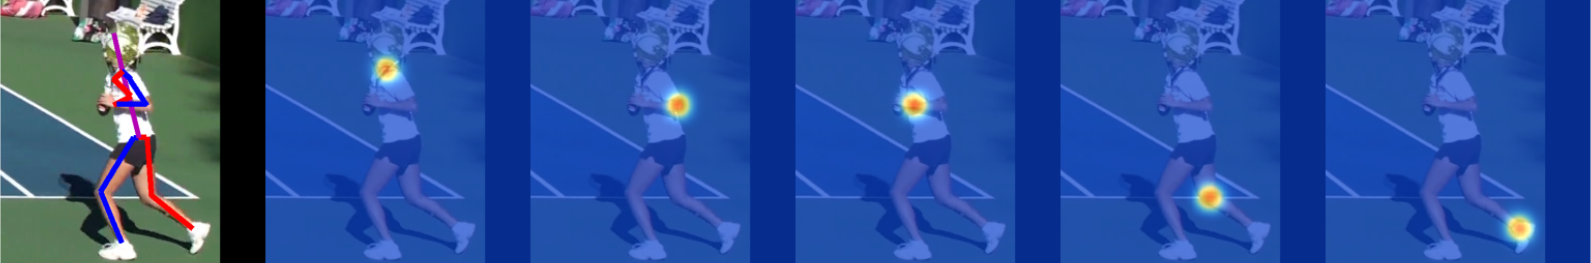
\includegraphics[width=0.9\textwidth]{2dheatmaps.png}
    \caption{Representing joint coordinates as probability heatmaps. From left to right: Tree structure representation of all joints, left shoulder, left elbow, left hand, right knee and right ankle. Image taken from \cite{newell_stacked_2016}}
    \label{fig:probability-heatmaps}
\end{figure}

The skeleton structure shown is just a visualization of the data generated.
When computing pose, two main approaches are used.
Firstly, many approaches use regression to directly compute the image coordinates.
This approach was used in the early work because its reasoning is intuitive.
Secondly, heatmaps are used which represent a discrete probability distribution over the $x$ and $y$ coordinates.
One 2D heatmap corresponds to the position of one joint.
An example is provided in \fref{fig:probability-heatmaps}.
According to \cite{luvizon_2d/3d_2018}, in practice, heatmap based methods are preferred because the regression methods are often sub-optimal and result in lower accuracy of joint positions.
In order to extract the joint coordinates from heatmaps, a post processing step like the \textit{argmax} is needed.

When computing pose from images, one obvious challenge is variety in appearance because of different choices in \textbf{clothing}.
Consider the difference between detecting elbows in a picture with a person wearing a T-shirt and a picture with a person wearing a jacket.
Not only is the naked elbow exposed in the first example but the overall shape of the person is distorted because of the thick fabric of the jacket in the second example.
This problem also applies when considering the substantial differences in human appearance based on height, weight etc.

Another challenge is \textbf{occlusion} and \textbf{self-occlusion}. Occlusion happens when another object is in the line of sight of the camera, occluding parts of or the whole joint.
Self-occlusion means that the subject in the image is positioned to the camera in such a way that their own body occludes the joints.
When occlusion happens, image-based methods need to infer the most likely position from context and (depending on the approach) their information about human anatomy.

When focusing on detecting the pose of a single human, other \textbf{humans in the background} might complicate the process because their joints could be wrongly recognized as belonging to the desired subject.
Consider again the examples provided in \fref{fig:tree-skeleton}.
It is easy to see how such errors can occur in crowded environments.

According to \cite{zhu_articulated_2016}, there are two general approaches for pose estimation.
First, in \textit{top-down pose estimation}, a generic model of a human is used as a starting point.
This model is then updated based on the information gathered from the images.
That way, there is always a model where all joints are present (i.e. occlusion is handled easily).
This approach, however, requires a priori assumptions about the human body and may lead to subpar results when these assumptions are not true (i.e. people with disabilities, exceptionally tall or heavy people etc.).
Second, \textit{bottom-up pose estimation} focuses on detecting individual body parts.
These individual parts can then be combined together into the final pose representation.
Because part detectors got significantly more accurate in recent years due to the development of \textit{deep convolutional neural networks} this is the predominant approach for pose estimation in the current literature and also the approach of all methods presented in detail later.

\section{Neural Networks}
\label{sec:neural_networks}
Neural networks are becoming increasingly popular in modern computer vision and machine learning pipelines due to their high classification accuracy achieved by using deep architectures.
In the following chapter, an introduction into their functionality is given, as well as an outline of how they learn from data.

\subsection{Artificial Neural Networks}

\subsubsection{McCulloch-Pitts-Neuron}
One early approach for neural networks inspired by the human neuron was proposed by Warren McCulloch and Walter Pitts in 1943.
The McCulloch-Pitts-Neuron (MCP), also referred to as the McCulloch-Pitts unit, takes binary input values $\bm{x} = (x_1, \dots, x_n) \in \mathbb{B}^n$ and computes a binary value $f(\bm{x})$.
Additionally, the neuron contains a threshold value $\theta \in \mathbb{N}$.
After adding all input signals, the sum (also referred to as \textit{excitation}) is compared to $\theta$ \eref{eq:mcculloch-binary}.

\begin{equation}
    \begin{split}
        \label{eq:mcculloch-binary}
        f(\bm{x}, \theta)
        &=
        \begin{cases}
            1 & \text{if } \sum_{i=0}^n x_i \geq \theta \\
            0 & \text{otherwise}
        \end{cases}
%        \\
%        &= \phi(\psi(\bm{x}), \theta)
    \end{split}
\end{equation}

Even this simple neuron is capable of realizing some binary operators by choosing different values for $\theta$.
For example, the \textbf{boolean OR} operator is realized by setting $\theta = 1$ and the \textbf{boolean AND} operator can be implemented by choosing $\theta = n$.

A geometrical explanation of how the MCP works is that it separates its input space into two half-spaces, assigning the output $1$ to all input combinations on one side and $0$ on the other.
For example, for two dimensional input spaces (two input variables $x_1$ and $x_2$) this means that a MCP defines a separating line while for three dimensional input spaces the MCP becomes a separating hyperplane.
A visualization for the \textbf{boolean OR} function with three input variables is shown in \fref{fig:mcp-geometric-or}

\begin{figure}[htb!]
    \centering
    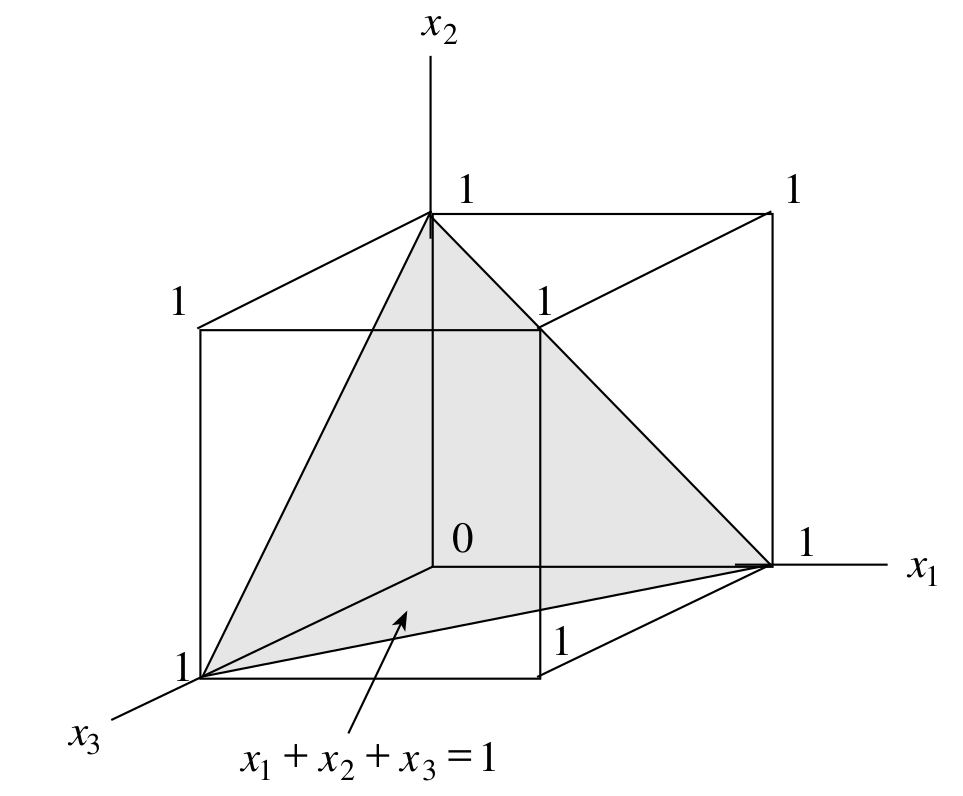
\includegraphics[width=0.6\textwidth]{mcp-geometric-or.png}
    \caption{Example of MCP dividing the three-dimensional input space using a hyperplane. The MCP is configured to model the \textbf{boolean OR} function. Image taken from \cite{rojas_neural_1996}}
    \label{fig:mcp-geometric-or}
\end{figure}

The MCP looked at so far is also called an \textit{uninhibited} MCP.
\cite{rojas_neural_1996} show that \textit{uninhibited} MCP's can only model monotonic logical functions.
By adding \textit{inhibitory inputs} $\bm{y} = (y_1, \dots, y_m) \in \mathbb{B}^m$ to the MCP, however, non-monotonic logical functions like \textbf{boolean NOT} can be implemented.
The output of the MCP changes to

\begin{equation}
    \hat{f}(\bm{x}, \bm{y}, \theta) = f(\bm{x}, \theta) \cdot \prod_{j = 0}^m (1 - y_j)
\end{equation}

Because of this definition it is possible to incorporate negated input values into the unit, giving it the ability to model a combination of negated and non-negated inputs aggregated with the \textbf{boolean AND} operator.
For example, modeling the boolean function $x_1 \wedge \neg x_2 \wedge x_3$ results to

\begin{equation}
    \hat{f}(x_1, x_2, x_3, \theta=1) = f(x_1, x_3, \theta) \cdot (1 - x_2)
\end{equation}

By using two layers of units where the first layer models conjunctions just as presented above and the second layer models a simple \textbf{boolean OR} function over the outputs of the first layer it is possible to model any boolean function $f: \mathbb{B}^n \to \mathbb{B}$ because any such function can be represented in disjunctive normal form.

The obvious limitation of McCulloch-Pitts-Networks is that they are limited to the domain of logical functions.
Additionally, they have to be constructed rather than being able to learn the desired function because they rely on fixed connections to model relations between input variables.

\subsubsection{Perceptron}

In contrast to the McCulloch-Pitts-Neuron a Perceptron uses real valued inputs $\bm{x} = (x_1, \dots, x_n) \in \mathbb{R}^n$ as well as real valued weights $\bm{w} = (w_1, \dots, w_n) \in \mathbb{R}^n$ for each edge.

\begin{equation}
    f(\bm{x}, \bm{w}, \theta) =
    \begin{cases}
        1 & \text{if } \sum_{i=0}^n w_i \cdot x_i \geq \theta \\
        0 & \text{otherwise}
    \end{cases}
\end{equation}

Instead of setting $\theta$ as part of the neuron it is preferred to treat it as an additional trainable parameter.
To achieve this, a new fixed input value $x_b = 1$ with the corresponding weight $w_b = -\theta$ is added to the model and the previously \emph{internal} $\theta$ is fixed to $0$ \eref{eq:full-perceptron}.
This additional weight is called the \textit{bias} of the Perceptron.

\begin{equation}
    \label{eq:full-perceptron}
    f(\bm{x}, \bm{w}) =
    \begin{cases}
        1 & \text{if } ~ -w_b + \sum_{i=0}^n w_i \cdot x_i \geq 0 \\
        0 & \text{otherwise}
    \end{cases}
\end{equation}

For notational convenience, from now on the bias is assumed to be part of $\bm{w}$, i.e. $\bm{w} = (w_1, \dots, w_n, -\theta)$ and the additional input $x_b = 1$ is part of $\bm{x}$, i.e. $\bm{x} = (x_1, \dots, x_n, 1)$.

The \textit{excitation} of a Perceptron is still just a (weighted) linear combination.
This means that the Perceptron, like the MCP, separates the input space by a hyperplane.
In \fref{fig:perceptron-logic} examples for some common logical functions for two input variables are provided.

\begin{figure}[htb!]
    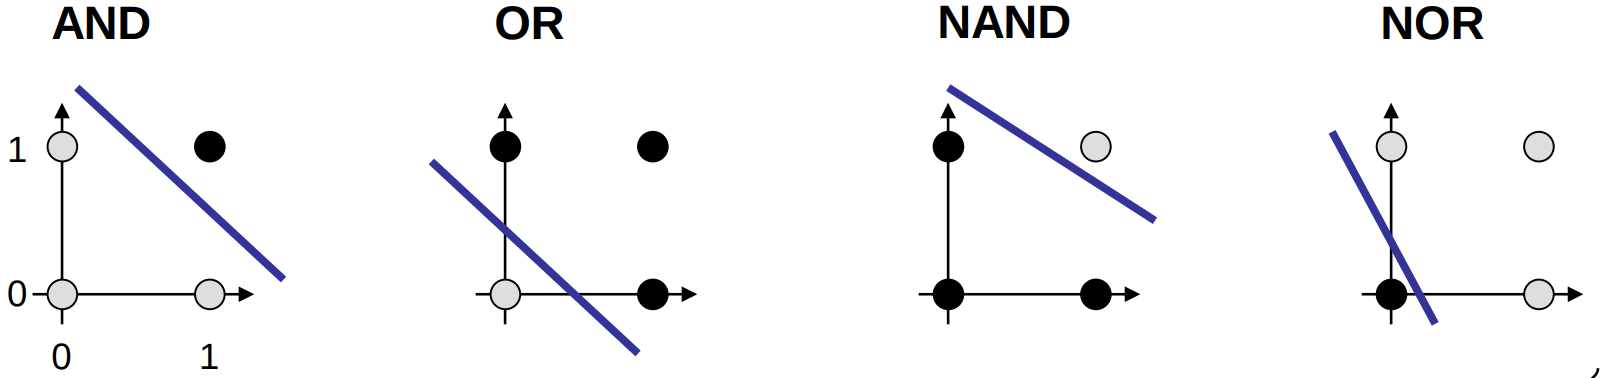
\includegraphics[width=0.9\textwidth]{perceptron-linear-seperable.png}
    \caption{Logical functions modelled by a single Perceptron. The blue line indicates where the input space is divided. All input combinations on one side of the line are going to be assigned to $1$ while being assigned to $0$ on the other side. Notice that there are infinitely many possibilities for dividing lines since the input space is real valued. Image taken from \cite{rudolph_lecture_2018}}
    \label{fig:perceptron-logic}
\end{figure}

While MCP's were designed to model logical functions like \textbf{boolean OR} or \textbf{boolean AND} by setting $\theta$ as well as categorizing the input variables as either \textit{inhibitory} or \textit{non-inhibitory}, Perceptrons are able to infer these parameters through a \textit{learning process}.

Learning in the context of Perceptrons means determining a parameter vector $\bm{w}$ which satisfies the following inequalities for all \textbf{positive points} $\bm{p} \in \bm{P}$ with $\hat{f}(\bm{p}, w) = 1$ as well as all \textbf{negative points} $\bm{n} \in \bm{N}$ with $\hat{f}(\bm{n}, w) = 0$

\begin{equation}
    \begin{split}
        \bm{w} \cdot \bm{p} &\geq 0 \\
        \bm{w} \cdot \bm{n} &< 0
    \end{split}
\end{equation}

A parameter vector which satisfies these inequalities then defines the hyperplane separating all positive negative points.

The general algorithmic approach for Perceptron learning is the following:
\begin{enumerate}
    \item Start with a random weight vector $\bm{w}$
    \item Evaluate how accurate the hyperplane defined by $\bm{w}$ separates the input space
    \item If all positive and negative points are separated correctly:
    \begin{enumerate}
        \item \textbf{Done}
    \end{enumerate}
    \item Else
    \begin{enumerate}
        \item Update weight vector in a way which further reduces the error function
        \item Go to step 2
    \end{enumerate}
\end{enumerate}

In order for the learning algorithm to determine the accuracy of a given weight vector $\bm{w}_i$ an \textbf{error function} or \textbf{loss function} needs to be provided.
Such a function takes all positive and negative points and calculates the amount of error (i.e. number of wrongfully classified points).
One example of an error function for binary functions is presented in \eref{eq:error-binary}\cite{rojas_neural_1996}.

\begin{equation}
    \label{eq:error-binary}
    E(\bm{w}_i) = \sum_{\bm{x} \in P} (1 - \hat{f}(\bm{x},\bm{w_i})) + \sum_{\bm{x} \in N} \hat{f}(\bm{x},\bm{w_i})
\end{equation}

It is trivial to see that the minimum error $E(\bm{w}) = 0$ is achieved if and only if $\hat{f}(\bm{x}) = 1$ for all positive points and $\hat{f}(\bm{x}) = 0$ else.

Iteratively updating the weight vector needs a strategy that guarantees that the error will be less than it was before after updating.
One algorithm, presented in \cite{rojas_neural_1996} and simply called \textit{Perceptron learning algorithm}, uses the following method.

\begin{figure}[htb!]
    \centering
    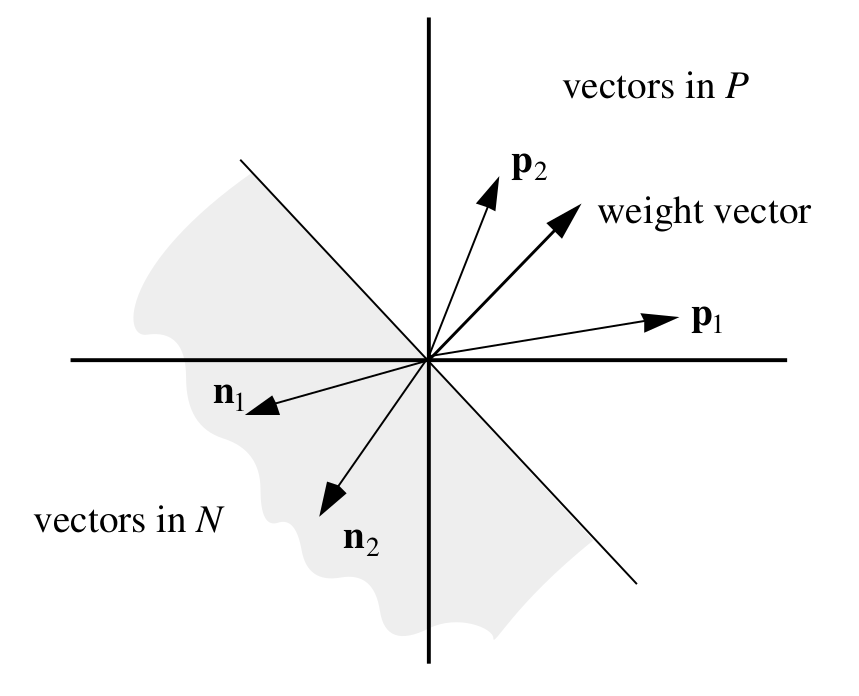
\includegraphics[width=0.55\textwidth]{perceptron-learning-update.png}
    \caption{Visualization of the weight plane $\bm{w} \cdot \bm{x}$ separating two positive and two negative vectors. The weight vector $\bm{w}$ is the normal of the hyperplane. Image taken from \cite{rojas_neural_1996}}
    \label{fig:perceptron-learning-update}
\end{figure}

Given the \textit{training data points} $M = P \cup N$, a point $x \in M$ is chosen randomly.
Also, as discussed before, a random weight vector $\bm{w}_t = \bm{w}_0$ is initialized.
If $x \in P$ and $\bm{w}_t \cdot x \leq 0$ then the weight vector needs to be updated.
The idea is that, in the case above, the two vectors $\bm{x}$ and $\bm{w}$ must have an angle bigger than 90 degrees (see \fref{fig:perceptron-learning-update}).
By rotating $\bm{w}$ towards $\bm{x}$ the angle will be reduced, eventually putting $\bm{x}$ on the correct side of the hyperplane.
In order to rotate $\bm{w}$ the algorithm proposes $\bm{w}_{t+1} = \bm{w}_{t} + \bm{x}$.
Analogously, if $x \in N$ and $\bm{w}_t \cdot x \geq 0$ the algorithm proposes $\bm{w}_{t+1} = \bm{w}_{t} - \bm{x}$.
This is done for each $x \in M$ in a random order.

Because $P$ and $N$ are linearly separable and there are a finite number of points it can be proven that, after a finite amount of steps, the error will be reduced to zero and the hyperplane will correctly separate the two sets \cite{rojas_neural_1996}.

\subsubsection{Gradient Descent Learning}

Another approach to learning the weights of a Perceptron is \textit{gradient descent}.
Given an error function $E$ with a set of initial weights $\bm{w_t}$ and an input point $\bm{x}$ the amount of error is given by $E(\bm{w}, \bm{x})$.
If the error function is differentiable one can calculate the gradient of the error function for each weight $w_i \in \bm{w}$ using

\begin{equation}
    \frac{\partial E}{\partial w_i}
\end{equation}

which points toward the steepest ascend of the error function.

Consider the error function defined earlier in \eref{eq:error-binary}.
The partial derivative given each $w_i \in \bm{w}$ is then given by

\begin{equation}
    \label{eq:error-derivative-1}
    \begin{split}
        \frac{\partial E(P \cup N, \bm{w})}{\partial w_i}
        &= \frac{\partial }{\partial w_i} \left( \sum_{x \in P} (1 - \hat{f}(\bm{x},\bm{w})) + \sum_{\bm{z} \in N} \hat{f}(\bm{z},\bm{w}) \right) \\
        &= \frac{\partial }{\partial w_i} \sum_{x \in P} (1 - \hat{f}(\bm{x},\bm{w})) + \frac{\partial }{\partial w_i} \sum_{\bm{z} \in N} \hat{f}(\bm{z},\bm{w}) \\
        &= \sum_{x \in P} \frac{\partial }{\partial w_i} (1 - \hat{f}(\bm{x},\bm{w})) + \sum_{\bm{z} \in N} \frac{\partial }{\partial w_i} \hat{f}(\bm{z},\bm{w}) \\
        &= \sum_{x \in P} - \frac{\partial }{\partial w_i} \hat{f}(\bm{x},\bm{w}) + \sum_{\bm{z} \in N} \frac{\partial }{\partial w_i} \hat{f}(\bm{z},\bm{w})
    \end{split}
\end{equation}

This presents a challenge, however.
Until now, the formal definition of a single Perceptron was

\begin{equation}
    \begin{split}
        \hat{f}(\bm{x}, \bm{w})
        &=
            \begin{cases}
                1 & \text{if } \bm{w} \cdot \bm{x} \geq 0 \\
                0 & \text{otherwise}
            \end{cases}
        \\
        &= \phi(\bm{x} \cdot \bm{w})
        \\
        &= \phi(\psi(\bm{x}, \bm{w}))
    \end{split}
\end{equation}

where $\psi$ is called the \textit{integration function} which computes the excitation and $\phi$ the \textit{activation function} which computes the activation of the neuron.

This results in a non-differentiable activation function since the thresholding approach is not continuous, it cannot be differentiable either.
A popular choice for a differentiable activation function is the \textit{sigmoid activation function} $S(x)$ given by

\begin{equation}
    S(x) = \frac{1}{1 + e^{-x}}
\end{equation}

One can easily see that the sigmoid function is differentiable and that the derivative is given by

\begin{equation}
    \begin{split}
        \frac{d}{dx} S(x)
        &= \frac{e^{-x}}{(1 + (e^{-x})^2)} \\
        &= S(x)(1 - S(x))
    \end{split}
\end{equation}

By then choosing $\phi = S$ and keeping $\psi(\bm{x}, \bm{w}) = \bm{x} \cdot \bm{w}$ in \eref{eq:error-derivative-1} the partial derivative of the error function becomes

\begin{equation}
    \label{eq:error-derivative-2}
    \begin{split}
        \frac{\partial E(P \cup N, \bm{w})}{\partial w_i}
        &= \sum_{x \in P} - \frac{\partial }{\partial w_i} \hat{f}(\bm{x},\bm{w}) + \sum_{\bm{z} \in N} \frac{\partial }{\partial w_i} \hat{f}(\bm{z},\bm{w})  \\
        &=  \sum_{x \in P} - \frac{\partial }{\partial w_i} \psi(\phi(\bm{x},\bm{w})) + \sum_{\bm{z} \in N} \frac{\partial }{\partial w_i} \psi(\phi(\bm{z},\bm{w})) \\
        &=  - \sum_{x \in P} \frac{\partial }{\partial w_i} S(\bm{x} \cdot \bm{w}) + \sum_{\bm{z} \in N} \frac{\partial }{\partial w_i} S(\bm{z} \cdot \bm{w}) \\
        &=  - \sum_{x \in P}  S(\bm{x} \cdot \bm{w}) (1 - S(\bm{x} \cdot \bm{w})) + \sum_{\bm{z} \in N} S(\bm{z} \cdot \bm{w}) (1 - S(\bm{z} \cdot \bm{w}))\\
    \end{split}
\end{equation}

After computing the partial derivative for each $w_i \in \bm{w}$ the \textit{gradient} then is

\begin{equation}
    \nabla E(P \cup N, \bm{w}) = \left(\frac{\partial E(P \cup N, \bm{w})}{\partial w_1}, \dots, \frac{\partial E(P \cup N, \bm{w})}{\partial w_n} \right)
\end{equation}

Finally, the current weights $\bm{w_t}$ can be updated by changing the weights a certain \textit{step size or learning rate} $\gamma$ towards a local minimum of the error function by applying

\begin{equation}
    \label{eq:gradient-binary-update}
    \bm{w_{t+1}} = \bm{w_t} - \gamma ~ \nabla E(P \cup N, \bm{w_t})
\end{equation}

Since the gradient points toward the steepest ascent of the error function a negation is needed to approach the local minimum.

\subsubsection{Multi-Layer Perceptron}
Until now, the assumption was made that the two sets of points $P$ and $N$ are linearly separable.
Many problems, however, are more complex and cannot be easily separated linearly.
One example from the realm of logical functions is the \textbf{XOR} function.
As an example, consider \textbf{XOR} with two input variables.
If visualized in the same way as in \fref{fig:perceptron-logic} it is quite trivial to see that no single line is able to divide the positive from the negative points.
Therefor, a more complex model is necessary for modeling functions with \textit{convex solution spaces} such as \textbf{XOR} \fref{fig:xor-convex}.
This is achieved by grouping Perceptrons into \textit{layers} and connecting them together.

\begin{figure}[htb!]
    \centering
    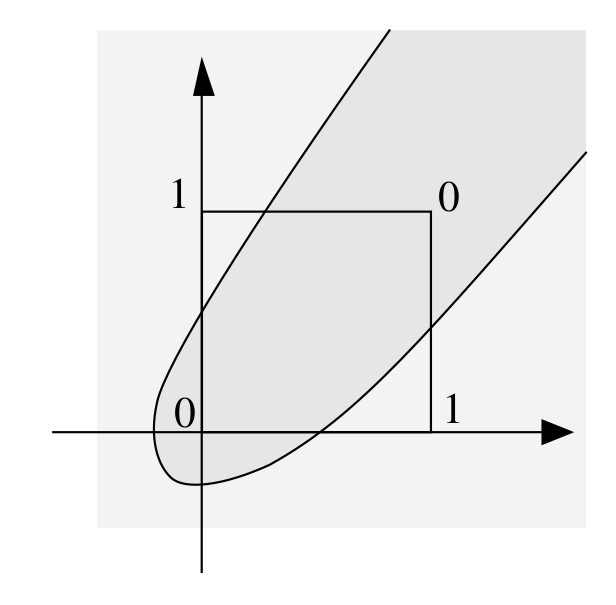
\includegraphics[width=0.5\textwidth]{xor-convex.png}
    \caption{Solving the \textbf{XOR} problem by using separating \textit{regions} instead of hyperplanes. Image taken from \cite{rojas_neural_1996}}
    \label{fig:xor-convex}
\end{figure}

Let $\bm{N} = (N_1, \dots, N_L)$ be a \textit{multi-layer perceptron (MLP)} consisting of $L$ layers.
From now on, for notational convenience, the term \textit{multi-layer perceptron} and \textit{neural network} are used interchangeably.
In the literature, sometimes the inputs are also considered to be a layer, even though they do not consist of Perceptrons.
This then means that a MLP has one input layer, several \textit{hidden layers} with the last hidden layer also providing the output.
When referring to the number of layers of a MLP only the hidden layer are counted, meaning that a MLP consisting of $L=3$ layer has one input layer and three hidden layer.

Each hidden layer $N_l$ consists of $m_l \in \mathbb{N}$ Perceptrons.
Consecutive layers are connected by directed, weighted edges $w_{ij} \in \mathbb{R}$ with $n_i \in N_l$ and $n_j \in N_{l+1}$ so that each Perceptron $n_i$ is connected to the input of each Perceptron $n_j$ in the consecutive layer.
Two Perceptrons inside the same layer are not allowed to be connected in traditional MLP definitions.
Also, the inputs to the MLP are only allowed to be connected to the first layer $N_1$.

By choosing $L=2$ a MLP is capable of modeling every convex solution space \cite{rojas_neural_1996}.
The Perceptrons in the first layer each learn to linearly separate the solution space into two parts like described earlier.
By using just one Perceptron in the second layer, which is able to learn the \textbf{boolean AND} function over all outputs from the previous layer it is possible to learn any convex solution space.
A visualization is provided in \fref{fig:convex-solution}.

\begin{figure}[htb!]
    \centering
    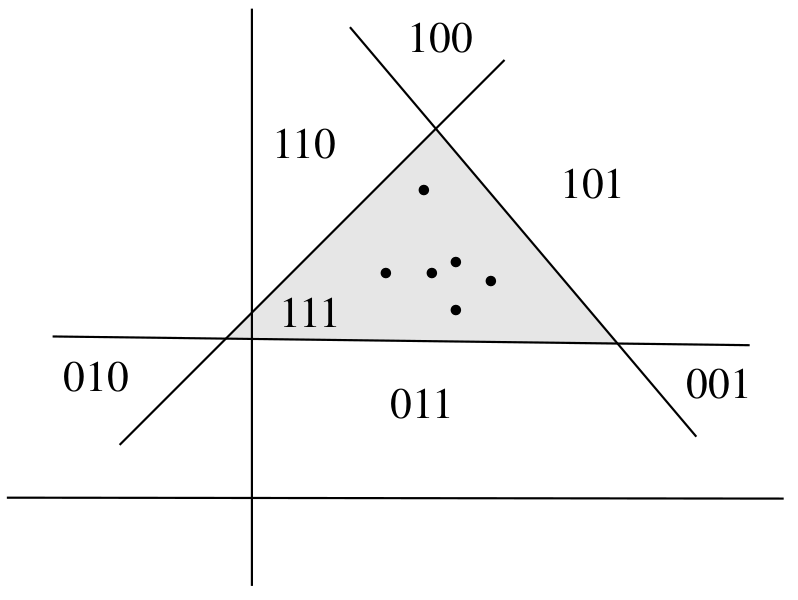
\includegraphics[width=0.8\textwidth]{convex_solution_space.png}
    \caption{Example of a convex solution space using a two-layered MLP with three Perceptrons in the first and one Perceptron in the second layer. Each bit vector $b = (x_1, x_2, _3)$ shows the output of Perceptron 1, 2 and 3 respectively. Image taken from \cite{rojas_neural_1996}}
    \label{fig:convex-solution}
\end{figure}

Even with the ability to model any convex solution space, there are still problems which have a \textit{non-convex solution space}.
However, by adding another layer to the MLP ($L=3$) these problems can also be solved.

The first hidden layer behaves just like in the previous example with each Perceptron splitting the input space into two.
Each Perceptron in the second layer again learns \textbf{boolean AND} functions, resulting in $\lVert N_2 \rVert$ convex regions.
In the third layer, a Perceptron then combines these regions into non-convex regions using the learned \textbf{boolean OR} operator.
In fact, a three-layer MLP is able to model any arbitrary function (given enough Perceptrons per layer).

These intuitive ideas of how the MLP is able to model any arbitrary function does not imply, however, that each Perceptron in the third layer \textit{has} to learn the \textbf{boolean OR} function etc.
They just show that these MLPs are powerful enough to model any arbitrary function by combining simple features (separating hyperplanes) from previous layers to form new, more complex features (combinations of convex regions) with each consecutive layer.

\subsubsection{Backpropagation}

Probably the most common learning algorithm for training MLPs is the \textbf{backpropagation algorithm}, initially proposed by Paul Werbos in 1974 and popularized by Rumelhart, Hinton and Williams in 1986.
It uses gradient descent with the addition of propagating the error backwards through the network by making use of the chain rule of derivation.

For each point $\bm{x_i}$ in the training data, the algorithm follows these steps:

\begin{enumerate}
    \item Start with random weights $\bm{W}_0 = (\bm{w_{1_0}}, \dots, \bm{w_{N_0}})$ for each neuron.
    \item Pass $\bm{x_i}$ into the network (called a \textit{forward pass})
    \begin{itemize}
        \item $\hat{f}(\bm{x_i}, \bm{w}_0) = \bm{y_i}$
    \end{itemize}
    \item Compute gradient at the last layer by using a loss function and the expected result $\hat{\bm{y_i}}$.
    \item Compute gradient for the previous layers, incorporating the error from the consecutive layers (called a \textit{backward pass}).
    \item Update the weights with their corresponding gradients.
\end{enumerate}

In order to show how the Backpropagation algorithm works consider a MLP with $L=2$ hidden layers $L_1, L_2$ and $\left| \bm{x} \right| = N$ inputs.
Also, let $\lVert L_1 \rVert = \lVert L_2 \rVert = M$ without loss of generality.

First, the forward pass is performed.
The output of each neuron $h_j(\bm{x}, \bm{w_j}) = y_j$ in the first hidden layer can be described using the following equation

\begin{equation}
    \begin{split}
        h_j(\bm{x}, \bm{w_j})
        &= S(\bm{x} \cdot \bm{w_j}) \\
        &= \frac{1}{1 + e^{-(\bm{x} \cdot \bm{w_j})}}
    \end{split}
\end{equation}

Similarly, after the second layer, the output $g_k$ for each neuron given the network input can be described as

\begin{equation}
    \begin{split}
        g_k(\bm{x}, \bm{w_k})
        &= S\left(\sum_{j=0}^M w_{jk} \cdot h_j(\bm{x}, \bm{w_j})\right) \\
        &= S\left(\sum_{j=0}^M w_{jk} \cdot S \left(\sum_{i=0}^N w_{ij} \cdot x_i\right)\right)
    \end{split}
\end{equation}

For notational convenience, instead of \eref{eq:error-binary}, consider the following loss function.
Every differentiable loss function can be used in the Backpropagation algorithm.

\begin{equation}
    SSE(\bm{w}) = \sum_{\bm{x} \in B} (\hat{f}(\bm{x}, \bm{w}) - y_x)^2
\end{equation}

This loss function, the \textbf{sum of squared errors}, computes the output of the Perceptron $\hat{f}(\bm{x}, \bm{w})$ for a given weight vector $\bm{w}$ and subtracts the expected output $y_x$ for the input $\bm{x}$.
By computing the square of the result the error value will be positive and larger errors will contribute more towards the error sum.

After the forward pass through the network the loss for a single output neuron $g_k$ is given by

\begin{equation}
    \begin{split}
        SSE(\bm{x}, (\bm{w_j}, \bm{w_k}))
        &= (y_k - \hat{y}_{k})^2 \\
        &= (g_k(\bm{x},\bm{w_k}) - \hat{y}_{k})^2 \\
        &= \left(S \left(\sum_{j=0}^M w_{jk} \cdot h_j(\bm{x}, \bm{w_j})\right) - \hat{y}_{k}\right)^2 \\
        &=  \left( S\left(\sum_{j=0}^M w_{jk} \cdot S \left(\sum_{i=0}^N w_{ij} \cdot x_i\right)\right) - \hat{y}_{k}\right)^2
    \end{split}
\end{equation}

By using the same approach as with gradient descent, the partial derivative of the loss function with regards to the weights of the second layer is given by

\begin{equation}
    \begin{split}
        \frac{\partial ~ SSE(\bm{x}, \bm{w})}{\partial w_{jk}}
        &= \frac{\partial}{\partial w_{jk}} (g_k(\bm{x},\bm{w_k}) - \hat{y}_{k})^2
    \end{split}
\end{equation}

Using the chain rule for derivation

\begin{equation}
    (p(b(x)))' = p'(b(x)) \cdot b'(x)
\end{equation}

the partial derivative can be broken down into

\begin{equation}
    \begin{split}
        \frac{\partial ~ SSE(\bm{x}, \bm{w})}{\partial w_{jk}}
        &= \frac{\partial}{\partial w_{jk}} ~ (g_k(\bm{x},\bm{w_k}) - \hat{y}_{k})^2 \\
        &= 2 \cdot (g_k(\bm{x},\bm{w_k}) - \hat{y}_{k}) \cdot  S'\left(\sum_{j=0}^M w_{jk} \cdot h_j(\bm{x}, \bm{w_j})\right) \cdot h_j(\bm{x}, \bm{w}_j) \\
        &= 2 \cdot (y_k - \hat{y}_{k}) \cdot  y_k \cdot (1 - y_k) \cdot h_j(\bm{x}, \bm{w_j}) \\
        &= \delta_k \cdot h_j(\bm{x}, \bm{w_j}) \\
        &= \delta_k \cdot y_j
    \end{split}
\end{equation}

One can observe that the output of all neurons from layer $N_{k}$ are needed to compute the partial derivate for neurons in layer $N_{k+1}$, which is why the initial forward pass through is necessary.

Similarly, the partial derivative of the loss function with regards to $w_{ij}$ is given by \eref{eq:backprop-partial-hidden}.
However, while running Backpropagation, the partial derivatives of all nodes in layer $N_{k+1}$ need to be computed first in order to determine the partial derivative of nodes in layer $N_{k}$ \cite{rojas_neural_1996}.

\begin{equation}
    \label{eq:backprop-partial-hidden}
    \begin{split}
        \frac{\partial ~ SSE(\bm{x}, \bm{w})}{\partial w_{ij}}
        &= \frac{\partial}{\partial w_{ij}} ~ (g_k(\bm{x},\bm{w_k}) - \hat{y}_{k})^2 \\
        &= 2 \sum_{k=0}^{K} (g_k(\bm{x},\bm{w_k}) - \hat{y}_{k}) \cdot  S'\left(\sum_{j=0}^M w_{jk} \cdot h_j(\bm{x}, \bm{w_j})\right) \cdot w_{jk} \cdot S'(\bm{x} \cdot \bm{w_j}) \cdot x_i \\
        &= 2 \sum_{k=0}^{K} (g_k(\bm{x},\bm{w_k}) - \hat{y}_{k}) \cdot  g_k(\bm{x},\bm{w_k}) \cdot (1-g_k(\bm{x},\bm{w_k})) \cdot w_{jk} \cdot h_j(\bm{x}, \bm{w_j}) \cdot (1-h_j(\bm{x}, \bm{w_j})) \cdot x_i \\
        &= 2 \sum_{k=0}^{K} (y_k - \hat{y}_{k}) \cdot  y_k \cdot (1-y_k) \cdot w_{jk} \cdot y_j \cdot (1-y_j) \cdot x_i \\
        &= x_i \cdot y_j \cdot (1-y_j) \cdot \sum_{k=0}^{K} 2 \cdot (y_k - \hat{y}_{k}) \cdot y_k \cdot (1 - y_k) \cdot w_{jk} \\
        &= x_i \cdot y_j \cdot (1-y_j) \cdot \sum_{k=0}^{K} \delta_k \cdot w_{jk} \\
        &= x_i \cdot \delta_j
    \end{split}
\end{equation}

Generally, the error signal $\delta$ can be computed like this for all layer $L_g$ in the network:

\begin{equation}
    \delta_j =
    \begin{cases}
        y_j \cdot (1 - y_j) \cdot (y_j - \hat{y}_j) & ~ \text{if} ~ L_g ~ \text{is output layer} \\
        y_j \cdot (1 - y_j) \cdot \sum_{k \in L_{g+1}} \delta_k \cdot w_{jk} & ~ \text{else}
    \end{cases}
\end{equation}

After computing the error signal, the weight can be updated, similarly to \eref{eq:gradient-binary-update}, using the following formula:

\begin{equation}
    \begin{split}
        w_{jk_{(t+1)}}
        &= w_{jk_{(t)}}  - \gamma \cdot \delta_k \cdot y_j
    \end{split}
\end{equation}

One problem that held the development of deep networks with many hidden layers back is the \textbf{vanishing gradient} problem.
As seen previously, part of the gradient that gets propagated back through the network to update the parameters is the derivative of the activation function.
When choosing Sigmoid as the activation function, the following can be easily shown:

\begin{equation}
    \frac{dS(x)}{dx} \leq 0.25
\end{equation}

A similar behaviour is true for many other activation functions like $tanh(x)$.
Thus, when multiplying many of such gradients together the overall gradient \textit{vanishes}, which means that the layers towards the beginning of the network are not trained efficiently.

One way of dealing with this problem is using the \textbf{Rectified Linear Unit} non-linearity as activation function, as proposed in \cite{nair_rectified_2010}:

\begin{equation}
    \text{ReLU}(x) = \max (0, x)
\end{equation}

When computing the derivative of \textbf{ReLU}, it becomes clear that the vanishing gradient problem cannot occur because the gradient is either propagated completely or not at all as opposed to being diminished with every layer:

\begin{equation}
    \frac{d \text{ReLU}(x)}{dx} = \begin{cases}
        1 & if ~ x > 0 \\
        0 & if ~ x < 0
    \end{cases}
\end{equation}

\subsection{Convolutional Neural Networks}
Suppose a task like image classification should be performed using traditional artificial neural networks like described previously.
In image classification, images get sorted into classes based on what their content is, for example, an image of a cat should be classified to be of class \textit{cat} etc.
For simplicity, consider the image to be greyscale, which means that each pixel $x$ contains the overall brightness information represented as a single byte (i.e. $x \in [0,255] \subset \mathbb{N}_0$).

In order to use the image as an input, one would pass each pixel as one input into the neural network.
For an image of size $n \times m$, this would mean a total of $n \cdot m$ neurons in the input layer.
Let the following hidden layer consist of $h$ neurons.
This then means that there need to be $(n \cdot m) \cdot h$ weights for the first hidden layer alone.
One can see that, even for small images consisting of $32 \times 32$ pixels, the number of weights increase dramatically.

\subsubsection{Convolutional Layer}

Instead of using traditional neural network layers for images, \textbf{convolutional layers} can be used.
They relate to the mathematical process of convolution, where two real-valued functions are combined using the convolution operator $*$, resulting in a third real-valued function.
In its most general form, the convolution operator over functions $x(t)$ and $w(a)$ is defined in \cite{goodfellow_deep_2016} as:

\begin{equation}
    s(t) = (x * w)(t) = \int x(a)w(t-a)da
\end{equation}

In convolutional layers, a discretized version is employed.
The two operands are the input image $\bm{I}$ and a \textbf{kernel} (also referred to as a \textbf{filter}) $\bm{K}$.
Typically, a kernel is a quadratic two dimensional matrix $(p \times p)$ of weights $w_{ij} \in \mathbb{R}$ with $p$ being odd \eref{eq:kernel_definition}.

\begin{equation}
    \label{eq:kernel_definition}
    \bm{K} =
    \begin{pmatrix}
        w_{00} & \dots  & w_{0p} \\
        \vdots & \ddots & \\
        w_{p0} &        & w_{pp}
    \end{pmatrix}
\end{equation}

For each index $(i,j)$ in the input image, the output of the convolution is the weighted sum of the surrounding pixels of $(i,j)$:

\begin{equation}
    \begin{split}
        (\bm{K} * \bm{I})(i,j)
        &= \sum_{n=-s}^s \sum_{m=-s}^s \bm{K}_{(m+s, n+s)} \cdot \bm{I}_{(i+s, j+s)} \\
        &= \sum_{n=-s}^s \sum_{m=-s}^s w_{m+s, n+s} \cdot \bm{I}_{(i+s, j+s)}
    \end{split}
\end{equation}

with $s = \lfloor \frac{p}{2} \rfloor$.
A visualization of this process can be seen in \fref{fig:conv-vis}.
Repeating this process for each $(i,j)$ then produces a \textit{output feature map}.
A neural network with at least one convolutional layer is also often referred to as a \textbf{convolutional neural network} of a \textbf{CNN}.

\begin{figure}[htb!]
    \centering
    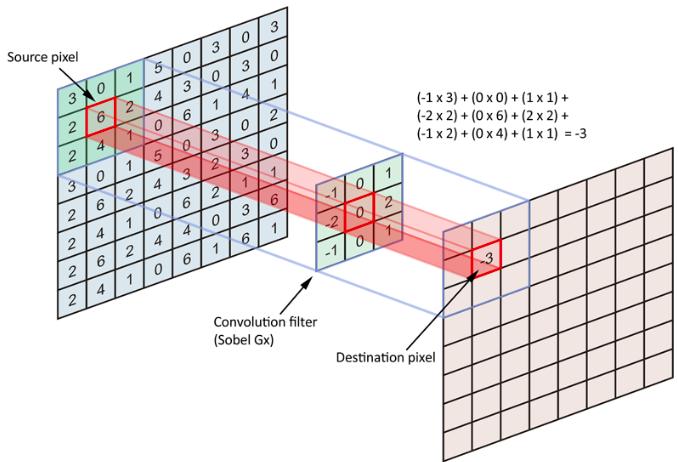
\includegraphics[width=0.8\textwidth]{conv-freecodecamp}
    \caption{Visualisation of one step of a convolutional layer. Image taken from \cite{dertat_applied_2017}}
    \label{fig:conv-vis}
\end{figure}

In practice, each convolutional layer consists of multiple kernels, each with distinct weights.
This results in a output feature map with a depth corresponding to the number of different kernels.
Also, the output feature map of a convolutional layer can be processed by another convolutional layer, which lets a convolutional neural network combine features by stacking convolutional layers on top of each other.

According to \cite{goodfellow_deep_2016}, convolutional layers have three important properties to consider.

\begin{figure}[htb!]
    \centering
    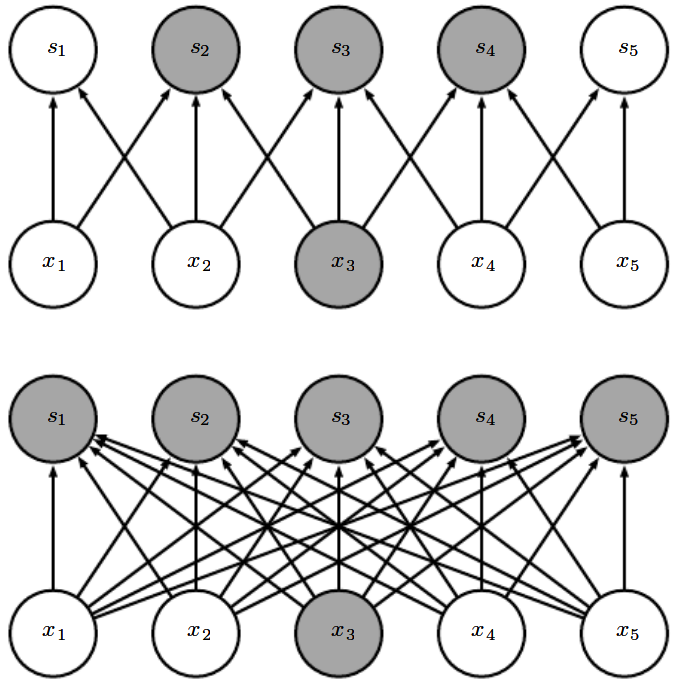
\includegraphics[width=0.8\textwidth]{sparse-connectivity.png}
    \caption{A visualization of sparse connectivity. Bottom: Connections in a traditional Multi-layer Perceptron. The output of each neuron is connected to the input of all neurons in the successive layer. Top: Connectivity in the case of a three-dimensional kernel. Each neuron is used just three times in order to compute the output of a neuron in the next layer. Image taken from \cite{goodfellow_deep_2016}}
    \label{fig:sparse-connectivity}
\end{figure}

Firstly, a convolution layer utilizes \textbf{sparse connectivity}.
This means that not all inputs are connected to all neurons in the next layer.
To illustrate this, consider a one dimensional input vector $\bm{x}$ and a kernel $\bm{k} \in \mathbb{R}^p$.
By calculating $(\bm{k} * \bm{x})(i)$ for each entry $i$ it becomes clear that each input $\bm{x}_i$ is only used to calculate $p$ output values.
See \fref{fig:sparse-connectivity} for a visualization.
Because of this property, the amount of parameters needed reduces drastically.
Traditionally, $m \cdot n$ parameters would be needed to calculate all output values for $m$ inputs and $n$ neurons.
Using convolutions, this reduces to $m \cdot p$.

Secondly, \textbf{parameter sharing} is another important property of convolutional layers.
Convolutions do not learn one weight per input but a fixed amount of weights defined by the kernel size.
Because there are only $p^2$ parameters to learn (assuming a two dimensional kernel) as opposed to $m \cdot n$ this further reduces the number of needed parameters.

Thirdly, convolution layer are \textbf{equivariant to translation}.
This means that changes in the input result in the same change in the output.
More specifically, translating the input and then calculating the convolution results in the same output as calculating the convolution first and then applying translation.
This is useful when considering that a kernel can easily learn to detect edges in the input image.
Without this property, it would not be guaranteed that the edge detector produces the same output no matter where in the image an edge is occurring.

% padding
Until now, it was assumed that the kernel can be applied on every image index $(i,j)$.
For corner pixels, this cannot be the case, however, if the kernel size is bigger than $1$, which is the case most of the times.
This then means that the output would be smaller in dimension because the corner pixels need to be omitted in order to calculate the convolution.

Padding fills in the missing values when calculating convolutions.
One popular approach is to fill the missing values with $0$. Consider the following example for a $(3,3)$ kernel at the image position $(i,j) = (0,0)$, which is defined as the top-left corner of the image:

\begin{equation}
    \begin{split}
        (\bm{K} * \bm{I})(i,j)
        &= w_{00} \cdot 0 + w_{01} \cdot 0 + w_{02} \cdot 0 \\
        &+ w_{10} \cdot 0 + w_{11} \cdot \bm{I}_{i,j} + w_{12} \cdot \bm{I}_{i+1,j} \\
        &+ w_{20} \cdot 0 + w_{21} \cdot \bm{I}_{i,j+1} + w_{22} \cdot \bm{I}_{i+1,j+1}
    \end{split}
\end{equation}

% stride ?


% receptive field ?

% stacking layers ?


\subsubsection{Pooling Layer}
Another important layer type when using Convolutional Neural Networks is a pooling layer.

\begin{figure}[htb!]
    \centering
    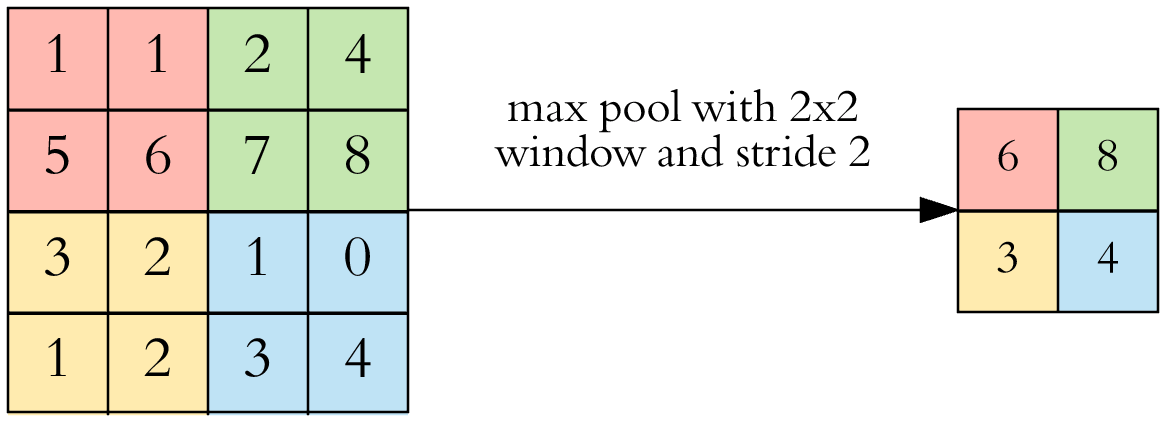
\includegraphics[width=0.8\textwidth]{pooling-tds.png}
    \caption{Example of a $2 \times 2$ Max-Pooling operation. Image taken from \cite{cornelisse_intuitive_2018}}
    \label{fig:pooling-tds}
\end{figure}

There are different types of pooling layer, however the most popular is the \textbf{Max-Pooling} layer where, for each $n \times n$ pixel block the maximum value is used as the output.
This then means that the size of the image is reduced.
For example, using a $2 \times 2$ Max-Pooling layer, the size is reduced by a factor of two in both dimensions.
See \fref{fig:pooling-tds} for a visualization.

Using a pooling layer, the representation becomes invariant to translations.
This means that small translations in an input image do not change the output of the pooling layer.
Pooling layers are useful if it is more important whether or not some feature is present in the image as opposed to finding the exact location.
For the task of image classification, for example, knowing that the image contains a face is more useful than to know the exact location of the face.

\begin{figure}[htb!]
    \centering
    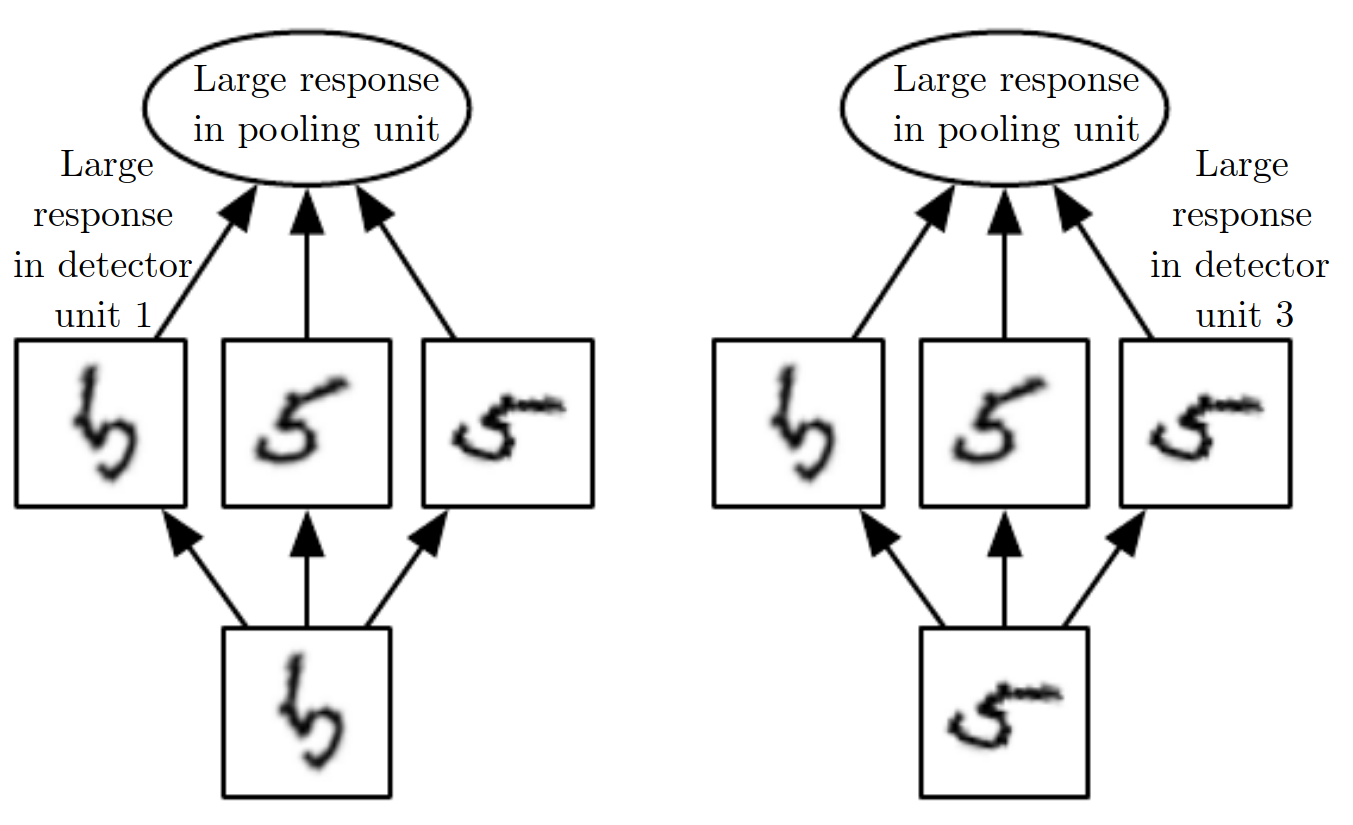
\includegraphics[width=0.8\textwidth]{pooling-goodfellow.png}
    \caption{Illustration of a Max-Pooling layer learning invariance towards rotation. By comparing the input against multiple differently rotated versions and just propagating the highest activation no matter which of the filters ultimately detected the number. Image taken from \cite{goodfellow_deep_2016}}
    \label{fig:pooling-goodfellow}
\end{figure}

This aspect of invariance towards translation is just an example, however.
Using a pooling layer, invariance towards specific characteristics can be learned.
Consider Fig. \ref{fig:pooling-goodfellow} where, using a pooling layer, invariance towards rotation is learned.

\subsubsection{Fully-Connected Layer}
In convolutional neural networks, the convolution and pooling layer produce a set of features.
Often, it is necessary to classify these features into categories.
Consider image classification or character recognition tasks as an example.
For this purpose, traditional layer of neurons like introduced earlier can be added to a convolutional neural network.
In the context of CNNs, these layers are referred to as \textbf{fully-connected} layers.
